%% Figure from MATH 556 notes, section 44 (Lecture 19). Board sketch (the diagonal process).
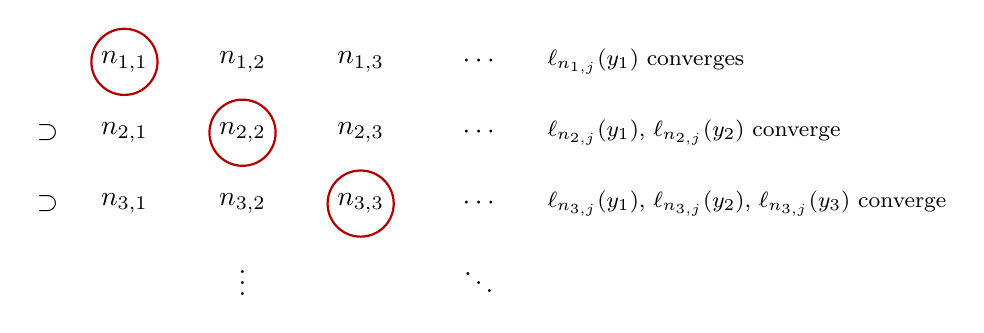
\begin{tikzpicture}[x=1.5cm, y=0.9cm]
  \foreach \k in {1,2,3} {
    \foreach \j in {1,2,3} \node at (\j,-\k) {$n_{\k,\j}$};
    \node at (4,-\k) {$\cdots$};
  }
  \node at (2,-4) {$\vdots$};
  \node at (4,-4) {$\ddots$};
  \foreach \k in {1,2,3} \draw[red!70!black, thick] (\k,-\k) circle (0.42cm);
  \foreach \k in {2,3} \node at (0.35,-\k) {$\supset$};
  \node[right, font=\footnotesize] at (4.5,-1) {$\ell_{n_{1,j}}(y_1)$ converges};
  \node[right, font=\footnotesize] at (4.5,-2) {$\ell_{n_{2,j}}(y_1)$, $\ell_{n_{2,j}}(y_2)$ converge};
  \node[right, font=\footnotesize] at (4.5,-3) {$\ell_{n_{3,j}}(y_1)$, $\ell_{n_{3,j}}(y_2)$, $\ell_{n_{3,j}}(y_3)$ converge};
\end{tikzpicture}
